% Provenance (never printed): BCPST year 1 geology (2021), "la carte
% geologique" (reading a map, structures, chronology), union licence
% Sciences de la Terre L1 (cartographie: strike and dip, three-point problem,
% outcrop patterns, DEM and GIS). See sources/outline_sources.md. Pilot
% chapter, 2026-10-22. The region is the series' invented Varden Hills
% (figdata/shared/region.py); every number about it is computed in
% figdata/bachelor-1/varden_maps.py or figdata/bachelor-1/v_rule.py.
\chapter{Mapas geológicos}\label{ch:b1:geological-maps}

Un geólogo atraviesa una serie de colinas bajas con una tabla de mapas, una libreta y una brújula
con clinómetro. Casi todo el terreno es hierba, bosque o campo arado; la roca aparece solo aquí y
allá, en la orilla de un arroyo, en un corte de carretera, en un peñasco. A partir de esas miradas
dispersas, y de la forma del terreno, el geólogo debe decir qué roca yace bajo cada metro cuadrado
de las colinas, cómo están inclinadas las capas, dónde están rotas y en qué orden ocurrió todo
ello. El resultado es un \omterm{def:b1:geological-maps:geological-map}{mapa geológico}: un dibujo plano que codifica un cuerpo de roca
tridimensional. Este capítulo explica cómo se hace un mapa de este tipo y cómo se lee: cómo se
miden y se calculan la \omterm{def:b1:geological-maps:attitude}{actitud} de una superficie, por qué la traza de una capa dibuja los motivos
que dibuja y cómo un mapa cuenta una historia. Sus ejemplos proceden de una región imaginaria,
pero geológicamente coherente, las colinas de Varden, que reaparece a lo largo de este libro.

\begin{recall}
Un mapa topográfico muestra el relieve con curvas de nivel, líneas de igual altitud; su escala
relaciona las distancias del mapa con las del terreno (libro 1, año 9). Las edades relativas se
deducen de la superposición (una capa es más joven que las capas que tiene debajo, salvo que la
sucesión esté invertida), del corte transversal (lo que corta a una roca es más joven que ella) y
de la inclusión (libro 1, año 7). Una falla es una fractura a lo largo de la cual se han desplazado
los dos bloques (libro 1, año 7); la geometría de los \omterm{def:b1:geological-maps:fold}{pliegues} y las fallas es el tema de
\cref{ch:b1:faults-folds-fabrics}.
\end{recall}

\section{Un mapa es un corte a través de tres dimensiones}\label{sec:b1:geological-maps:cut}

\begin{definition}[Mapa geológico]\label{def:b1:geological-maps:geological-map}
Un \emph{mapa geológico}\index{mapa geológico} muestra, en cada punto de la superficie del
terreno, la unidad de roca que yace allí bajo el suelo, con los \emph{contactos}\index{contacto (geológico)} ---las superficies que separan dos unidades--- y las estructuras (fallas, \omterm{def:b1:geological-maps:fold}{ejes de
pliegues}, \omterm{def:b1:geological-maps:attitude}{actitudes} de las capas) que las afectan. Una \emph{unidad cartográfica}\index{unidad cartográfica} es un cuerpo de roca que puede reconocerse y seguirse en el campo y que se dibuja
con un color; su \emph{afloramiento}\index{afloramiento} es la zona donde aparece en la superficie.
\end{definition}

\begin{definition}[Modelo digital de elevaciones]\label{def:b1:geological-maps:dem}
Un \emph{modelo digital de elevaciones}\index{modelo digital de elevaciones} es una malla de
altitudes del terreno, $z = g(x,y)$, en puntos regularmente espaciados. Un sistema de información
geográfica almacena estas mallas y las demás capas del mapa (\omterm{def:b1:geological-maps:geological-map}{contactos}, fallas, medidas, sondeos)
en un marco de coordenadas común, y calcula con ellas.
\end{definition}

\begin{proposition}[El afloramiento de un contacto]\label{prop:b1:geological-maps:intersection}
Sea el terreno la superficie $z = g(x,y)$ y un contacto la superficie
$z = c(x,y)$. La traza del contacto en el mapa es la curva
\[
  g(x,y) = c(x,y),
\]
la proyección sobre el plano horizontal de la intersección de las dos superficies;
la unidad que yace encima del contacto aflora donde $g > c$.
\end{proposition}

\begin{proof}
Un punto del mapa está sobre la traza si y solo si la superficie del terreno en ese punto pertenece
al contacto, es decir, $g(x,y) = c(x,y)$. Donde $g(x,y) > c(x,y)$, el terreno está por encima del
contacto: la roca de la superficie pertenece a la unidad que yace encima de él.
\end{proof}

\begin{remark}[Cómo se dibujan los mapas de este libro]\label{rem:b1:geological-maps:computed}
Esto es exactamente lo que hace un sistema de información geográfica para dibujar un mapa a partir
de un modelo tridimensional: evalúa $g - c$ en la malla de un \omterm{def:b1:geological-maps:dem}{modelo digital de elevaciones} y traza
las curvas donde cambia de signo. Los mapas de las colinas de Varden de este libro se dibujaron
así, a partir de un modelo geológico en el que cada superficie es conocida.
\end{remark}

\begin{omfigure}
\begin{tikzpicture}
\begin{axis}[axis equal image, xmin=0, xmax=10, ymin=0, ymax=8, width=0.82\linewidth,
  tick label style={font=\scriptsize}, xlabel={este (km)}, ylabel={norte (km)},
  label style={font=\small}, colormap/blackwhite, enlargelimits=false]
\addplot[matrix plot*, mesh/cols=101, point meta=explicit, shader=interp] table[x=x_km, y=y_km, meta=shade] {figdata/out/bachelor-1-varden_maps-shade.dat};
\addplot[contour, line width=0.25pt, opacity=0.7] table {figdata/out/shared-region-contours.dat};
\addplot[index contour, opacity=0.8] table {figdata/out/shared-region-index-contours.dat};
\addplot[river] table {figdata/out/shared-region-river.dat};
\end{axis}
\end{tikzpicture}

{\small Las colinas de Varden como \omterm{def:b1:geological-maps:dem}{modelo digital de elevaciones}: el terreno iluminado desde el
noroeste, con curvas de nivel cada \qty{50}{m} (más gruesas en \qty{250}{m} y \qty{500}{m}) y el
río, que fluye hacia el este.}
\end{omfigure}

\begin{omfigure}
\begin{tikzpicture}
\begin{axis}[axis equal image, xmin=0, xmax=10, ymin=0, ymax=8, width=0.82\linewidth,
  tick label style={font=\scriptsize}, xlabel={este (km)}, ylabel={norte (km)},
  label style={font=\small}]
\addplot[lith schist, draw=black, line width=0.3pt, even odd rule] table {figdata/out/shared-region-unit-schist.dat};
\addplot[lith granite, draw=black, line width=0.3pt, even odd rule] table {figdata/out/shared-region-unit-granite.dat};
\addplot[om lith={icsTriassic!35}{om sand}, draw=black, line width=0.3pt, even odd rule] table {figdata/out/shared-region-unit-sandstone.dat};
\addplot[om lith={icsJurassic!40}{om limestone}, draw=black, line width=0.3pt, even odd rule] table {figdata/out/shared-region-unit-limestone.dat};
\addplot[om lith={icsJurassic!15}{om shale}, draw=black, line width=0.3pt, even odd rule] table {figdata/out/shared-region-unit-shale.dat};
\addplot[om lith={icsCretaceous!35}{om limestone}, draw=black, line width=0.3pt, even odd rule] table {figdata/out/shared-region-unit-chalk.dat};
% the fault is drawn before the alluvium: the younger alluvial floor conceals it
\addplot[normal fault] table {figdata/out/shared-region-fault.dat};
\addplot[lith alluvium, draw=black, line width=0.3pt, even odd rule] table {figdata/out/shared-region-unit-alluvium.dat};
\addplot[contour, opacity=0.55] table {figdata/out/shared-region-contours.dat};
\addplot[river] table {figdata/out/shared-region-river.dat};
\pic at (axis cs:4.3,6.6) {strikedip={350.6}{12}};
\pic at (axis cs:2.2,6.6) {strikedip={189.3}{12}};
\pic at (axis cs:8.6,1.4) {northarrow};
\fill[black] (axis cs:6.6,0.35) rectangle (axis cs:7.1,0.5);
\fill[white] (axis cs:7.1,0.35) rectangle (axis cs:7.6,0.5);
\fill[black] (axis cs:7.6,0.35) rectangle (axis cs:8.1,0.5);
\fill[white] (axis cs:8.1,0.35) rectangle (axis cs:8.6,0.5);
\draw[black, line width=0.4pt] (axis cs:6.6,0.35) rectangle (axis cs:8.6,0.5);
\node[font=\footnotesize, above, inner sep=1.5pt, fill=white, fill opacity=0.8, text opacity=1] at (axis cs:7.6,0.5) {\qty{2}{km}};
\end{axis}
\end{tikzpicture}

\smallskip
\begin{tikzpicture}[font=\footnotesize]
\matrix[column sep=7pt, row sep=3pt, matrix of nodes, nodes={anchor=west}] {
  \tikz\draw[black!60, line width=0.4pt, lith alluvium] (0,0) rectangle (0.7,0.32); & aluvión (Cuaternario) &
  \tikz\draw[black!60, line width=0.4pt, om lith={icsCretaceous!35}{om limestone}] (0,0) rectangle (0.7,0.32); & creta (Cretácico, 90 Ma) \\
  \tikz\draw[black!60, line width=0.4pt, om lith={icsJurassic!15}{om shale}] (0,0) rectangle (0.7,0.32); & lutita (Jurásico, 165 Ma) &
  \tikz\draw[black!60, line width=0.4pt, om lith={icsJurassic!40}{om limestone}] (0,0) rectangle (0.7,0.32); & caliza (Jurásico, 180 Ma) \\
  \tikz\draw[black!60, line width=0.4pt, om lith={icsTriassic!35}{om sand}] (0,0) rectangle (0.7,0.32); & arenisca (Triásico, 245 Ma) &
  \tikz\draw[black!60, line width=0.4pt, lith granite] (0,0) rectangle (0.7,0.32); & granito (310 Ma) \\
  \tikz\draw[black!60, line width=0.4pt, lith schist] (0,0) rectangle (0.7,0.32); & esquisto (480 Ma) &
  \tikz\draw[normal fault] (0,0.16) -- (0.9,0.16); & falla normal (trazos en el bloque hundido) \\
};
\end{tikzpicture}

{\small El \omterm{def:b1:geological-maps:geological-map}{mapa geológico} de las colinas de Varden, con las curvas de nivel, el río, dos \omterm{def:b1:geological-maps:attitude}{actitudes}
medidas (línea de \omterm{def:b1:geological-maps:attitude}{rumbo} y trazo de \omterm{def:b1:geological-maps:attitude}{buzamiento}, con el \omterm{def:b1:geological-maps:attitude}{buzamiento} en grados) y la leyenda. Las
edades son las de las unidades de la región; la falla está oculta bajo el aluvión más joven del
fondo del valle.}
\end{omfigure}

\section{La actitud de un plano}

\begin{definition}[Rumbo, buzamiento y dirección de buzamiento]\label{def:b1:geological-maps:attitude}
Sea una superficie geológica ---un plano de estratificación, un contacto, una falla--- localmente
plana. Su \emph{rumbo}\index{rumbo} es la dirección de las rectas horizontales que contiene, dada
como \omterm{def:b1:spherical-astronomy:horizontal}{acimut} (grados en el sentido de las agujas del reloj desde el norte). Su
\emph{buzamiento}\index{buzamiento} $\delta$ es el ángulo entre el plano y la horizontal, medido en
el plano vertical perpendicular al rumbo, $0 \le \delta \le \ang{90}$. Su
\emph{dirección de buzamiento}\index{dirección de buzamiento} $\alpha$ es el \omterm{def:b1:spherical-astronomy:horizontal}{acimut} de la recta de
máxima pendiente descendente del plano. Juntos forman la \emph{actitud}\index{actitud (de un plano)}
del plano, que se escribe dirección de buzamiento/buzamiento, por ejemplo $080/12$.
\end{definition}

\begin{notation}[Rumbo según la regla de la mano derecha]\label{not:b1:geological-maps:rhr}
Un \omterm{def:b1:geological-maps:attitude}{rumbo} puede leerse en dos sentidos opuestos. La \emph{regla de la mano derecha} elige el que
hace que el plano buce hacia la derecha de un observador que mira a lo largo del \omterm{def:b1:geological-maps:attitude}{rumbo}: \omterm{def:b1:geological-maps:attitude}{rumbo}
$= \alpha - \ang{90}$ (módulo \ang{360}). En un mapa, el símbolo es una línea de \omterm{def:b1:geological-maps:attitude}{rumbo} con un
trazo corto que apunta hacia abajo de la pendiente, etiquetado con el \omterm{def:b1:geological-maps:attitude}{buzamiento}.
\end{notation}

\begin{omfigure}
\tdplotsetmaincoords{65}{125}
\begin{tikzpicture}[tdplot_main_coords, font=\small, scale=1.05]
  % the horizontal plane
  \fill[omSea!50] (-2.2,-1.6,0) -- (2.2,-1.6,0) -- (2.2,1.6,0) -- (-2.2,1.6,0) -- cycle;
  \draw[black!40] (-2.2,-1.6,0) -- (2.2,-1.6,0) -- (2.2,1.6,0) -- (-2.2,1.6,0) -- cycle;
  % the dipping plane: strike along y (north), dipping east (+x) at 30 degrees
  \fill[omLithLime!80, opacity=0.85] (-0.0,-1.6,0) -- (-0.0,1.6,0) -- (2.2,1.6,-1.27) -- (2.2,-1.6,-1.27) -- cycle;
  \draw[black!60] (0,-1.6,0) -- (0,1.6,0) -- (2.2,1.6,-1.27) -- (2.2,-1.6,-1.27) -- cycle;
  % strike line (horizontal, in both planes)
  \draw[omThm, line width=1.1pt] (0,-1.6,0) -- (0,1.6,0);
  % dip line and the horizontal below it, with the dip angle
  \draw[omDef, line width=1.1pt, -{Stealth[length=2.4mm]}] (0,0,0) -- (2.2,0,-1.27);
  \draw[black!60, densely dashed] (0,0,0) -- (2.2,0,0);
  \draw[black!60, densely dashed] (2.2,0,0) -- (2.2,0,-1.27);
  \draw[black] plot[domain=0:30, samples=16, variable=\t] ({0.8*cos(\t)}, 0, {-0.8*sin(\t)});
  \node[font=\footnotesize] at (1.05,0,-0.22) {$\delta$};
  % north arrow on the horizontal plane
  \draw[black, -{Stealth[length=2mm]}] (-1.8,-1.2,0) -- (-1.8,-0.3,0);
  \node[font=\footnotesize] at (-1.8,-0.05,0) {N};
\end{tikzpicture}
\begin{tikzpicture}[font=\small]
  \node[align=left, anchor=west, text width=5.2cm] at (0,0) {%
    \textcolor{omThm}{\rule[0.5ex]{0.6cm}{1.1pt}} rumbo: una recta horizontal del plano;\\[3pt]
    \textcolor{omDef}{\rule[0.5ex]{0.6cm}{1.1pt}} la recta de máxima pendiente del plano, cuyo acimut es la dirección de buzamiento;\\[3pt]
    el buzamiento es el ángulo entre esta recta y la horizontal (discontinua).};
\end{tikzpicture}

{\small Un plano de \omterm{def:b1:geological-maps:attitude}{rumbo} norte que buza \ang{30} hacia el este (\omterm{def:b1:geological-maps:attitude}{actitud} $090/30$), cortando un
plano horizontal según su línea de \omterm{def:b1:geological-maps:attitude}{rumbo}. No a escala.}
\end{omfigure}

\begin{proposition}[Ecuación de un plano buzante]\label{prop:b1:geological-maps:plane}
Con $x$ hacia el este, $y$ hacia el norte y $z$ hacia arriba, el plano de \omterm{def:b1:geological-maps:attitude}{dirección de buzamiento}
$\alpha$ y \omterm{def:b1:geological-maps:attitude}{buzamiento} $\delta$ que pasa por el punto $(x_0, y_0, z_0)$ es
\[
  z = z_0 - \tan\delta\,\bigl[(x - x_0)\sin\alpha + (y - y_0)\cos\alpha\bigr].
\]
\end{proposition}

\begin{proof}
El vector horizontal unitario que apunta en la \omterm{def:b1:geological-maps:attitude}{dirección de buzamiento} es
$\vec u = (\sin\alpha, \cos\alpha, 0)$ (el \omterm{def:b1:spherical-astronomy:horizontal}{acimut} se mide desde el norte, el eje $y$, hacia el
este, el eje $x$). A lo largo del \omterm{def:b1:geological-maps:attitude}{rumbo}, perpendicular a $\vec u$, el plano es horizontal; a lo
largo de $\vec u$ desciende $\tan\delta$ por unidad de distancia horizontal. La distancia horizontal
de un punto a la recta de \omterm{def:b1:geological-maps:attitude}{rumbo} que pasa por $(x_0, y_0)$, contada positiva hacia abajo de la
pendiente, es $(x-x_0)\sin\alpha + (y-y_0)\cos\alpha$, de donde sale la fórmula.
\end{proof}

\begin{theorem}[Actitud a partir de tres puntos]\label{thm:b1:geological-maps:three-point}
Sean $P_1, P_2, P_3$ tres puntos no alineados de un plano, y
$\vec n = \overrightarrow{P_1P_2} \times \overrightarrow{P_1P_3} =
(n_x, n_y, n_z)$, elegido con $n_z > 0$ (si no, sustitúyase $\vec n$ por $-\vec n$). Entonces el
\omterm{def:b1:geological-maps:attitude}{buzamiento} y la \omterm{def:b1:geological-maps:attitude}{dirección de buzamiento} del plano son
\[
  \delta = \arccos\frac{n_z}{\|\vec n\|}, \qquad
  \alpha = \text{el acimut del vector horizontal } (n_x, n_y),
\]
es decir, el ángulo $\alpha \in [\ang{0}, \ang{360})$ con
$\sin\alpha = n_x/\sqrt{n_x^2+n_y^2}$ y $\cos\alpha = n_y/\sqrt{n_x^2+n_y^2}$
(el plano es horizontal si $n_x = n_y = 0$).
\end{theorem}

\begin{proof}
$\vec n$ es perpendicular a dos vectores independientes del plano, luego es normal a él. El
\omterm{def:b1:geological-maps:attitude}{buzamiento} es el ángulo entre el plano y la horizontal, igual al ángulo entre sus normales, $\vec n$
y la vertical $\vec k$: $\cos\delta = \vec n \cdot \vec k / \|\vec n\| = n_z/\|\vec n\|$.
Por \cref{prop:b1:geological-maps:plane}, el plano es $z = \text{const} -
\tan\delta\,(x\sin\alpha + y\cos\alpha)$, es decir,
$\tan\delta\sin\alpha\,x + \tan\delta\cos\alpha\,y + z = \text{const}$; su normal hacia arriba es
proporcional a $(\tan\delta\sin\alpha,
\tan\delta\cos\alpha, 1)$, cuya parte horizontal apunta en la \omterm{def:b1:geological-maps:attitude}{dirección de buzamiento}
$\alpha$. Como $\vec n$ es un múltiplo positivo de esta normal, $(n_x, n_y)$ también apunta en la
\omterm{def:b1:geological-maps:attitude}{dirección de buzamiento}.
\end{proof}

\begin{method}[El problema de los tres puntos]\label{met:b1:geological-maps:three-point}
Para hallar la \omterm{def:b1:geological-maps:attitude}{actitud} de un contacto encontrado en tres sondeos (o visto en tres \omterm{def:b1:geological-maps:geological-map}{afloramientos}):
\begin{enumerate}
  \item para cada sondeo, tómese la altitud del contacto: la altitud del terreno menos la
        profundidad a la que se encontró el contacto;
  \item escríbanse los tres puntos $P_i = (x_i, y_i, z_i)$ en metros, con $x$ hacia el este y
        $y$ hacia el norte;
  \item calcúlese $\vec n = \overrightarrow{P_1P_2} \times
        \overrightarrow{P_1P_3}$ y hágase positivo $n_z$;
  \item aplíquese \cref{thm:b1:geological-maps:three-point}; dese la \omterm{def:b1:geological-maps:attitude}{actitud} como \omterm{def:b1:geological-maps:attitude}{dirección de
        buzamiento}/\omterm{def:b1:geological-maps:attitude}{buzamiento} y, si se pide, el \omterm{def:b1:geological-maps:attitude}{rumbo} según la regla de la mano derecha.
\end{enumerate}
Sobre el papel, el mismo problema se resuelve con curvas de igual altitud del plano: en la
recta que une el punto más alto y el más bajo, búsquese por proporción el punto a la altitud del
tercero; la recta que pasa por estos dos puntos de igual altitud es una línea de \omterm{def:b1:geological-maps:attitude}{rumbo}; el
\omterm{def:b1:geological-maps:attitude}{buzamiento} se deduce de la diferencia de altitud entre dos líneas de \omterm{def:b1:geological-maps:attitude}{rumbo} paralelas y de su
separación.
\end{method}

\begin{example}[El flanco oriental del anticlinal de Varden]\label{ex:b1:geological-maps:east}
% computed in figdata/bachelor-1/varden_maps.py (boreholes E1-E3)
Tres sondeos, E1 en $(4000, 6000)$, E2 en $(4600, 7200)$ y E3 en $(5100, 6400)$ (metros al este y
al norte de la esquina suroeste del mapa), encuentran la base de la caliza a las altitudes $174$,
$4$ y $\qty{-74}{m}$. Entonces $\overrightarrow{P_1P_2} = (600, 1200, -170)$,
$\overrightarrow{P_1P_3} = (1100, 400, -248)$; su producto vectorial es
$(-229\,600, -38\,200, -1\,080\,000)$, que apunta hacia abajo, así que
\[
  \vec n = (229\,600,\ 38\,200,\ 1\,080\,000).
\]
Así, $\cos\delta = 1\,080\,000/\|\vec n\| \approx
0.9776$, $\delta \approx \ang{12.2}$, y la \omterm{def:b1:geological-maps:attitude}{dirección de buzamiento} es el \omterm{def:b1:spherical-astronomy:horizontal}{acimut} de
$(229\,600, 38\,200)$, $\alpha \approx \ang{80.6}$: la \omterm{def:b1:geological-maps:attitude}{actitud} es
$081/12$, con \omterm{def:b1:geological-maps:attitude}{rumbo} $\ang{351}$ según la regla de la mano derecha. La base de la caliza buza
suavemente hacia el este-nordeste.
\end{example}

\section{Patrones de afloramiento}

\begin{proposition}[Contactos horizontales y verticales]\label{prop:b1:geological-maps:hv}
La traza de un contacto horizontal sigue la curva de nivel de su altitud. La traza de un contacto
vertical es una recta en el mapa, sea cual sea el relieve.
\end{proposition}

\begin{proof}
Para $c(x,y) = z_0$, la traza $g(x,y) = z_0$ es la curva de nivel $z_0$
(\cref{prop:b1:geological-maps:intersection}). Un plano vertical es el conjunto de puntos cuya
posición horizontal está sobre una recta, a cualquier altitud; su traza en el mapa es esa recta.
\end{proof}

\begin{theorem}[La regla de la V]\label{thm:b1:geological-maps:v-rule}
Un contacto plano cruza un valle cuyo fondo desciende aguas abajo con pendiente $s > 0$. Sea $a$ la
tangente del \omterm{def:b1:geological-maps:attitude}{buzamiento} aparente del contacto en la dirección aguas abajo ($a > 0$ si buza hacia
aguas abajo, $a < 0$ si buza hacia aguas arriba, $a = 0$ si es horizontal). Entonces la traza del
\omterm{def:b1:geological-maps:geological-map}{afloramiento} dibuja una V cuyo vértice está en el fondo del valle y
\begin{itemize}
  \item apunta \emph{aguas abajo} si $a > s$: el contacto buza hacia aguas abajo más deprisa de lo
        que desciende el fondo del valle;
  \item apunta \emph{aguas arriba} si $a < s$: el contacto es horizontal, buza hacia aguas arriba,
        o buza hacia aguas abajo menos deprisa que el fondo.
\end{itemize}
Un contacto vertical no dibuja ninguna V.
\end{theorem}

\begin{proof}
Sea $\xi$ la distancia medida aguas abajo a lo largo del fondo del valle. El fondo está a la
altitud $z_g(\xi) = z_0 - s\xi$; en la sección vertical a lo largo del valle, el contacto está en
$z_c(\xi) = c - a\xi$. En el fondo, la traza está donde $z_g = z_c$:
\[
  \xi_{\text{fondo}} = \frac{c - z_0}{a - s}.
\]
En un flanco del valle, en un punto más alto que el fondo en $h > 0$ y a la misma distancia del
nacimiento del valle, el terreno está en $z_0 - s\xi + h$, así que la traza está donde
$c - a\xi = z_0 - s\xi + h$:
\[
  \xi_{\text{flanco}} = \frac{c - z_0 - h}{a - s}, \qquad
  \xi_{\text{fondo}} - \xi_{\text{flanco}} = \frac{h}{a - s}.
\]
Si $a > s$, la traza queda más aguas abajo en el fondo que en los flancos: la V apunta aguas
abajo. Si $a < s$, ocurre lo contrario. Un contacto vertical cruza el fondo y los flancos en el
mismo $\xi$.
\end{proof}

\begin{omfigure}
\begin{tikzpicture}
\pgfplotsset{vpanel/.style={axis equal image, xmin=-1, xmax=1, ymin=0, ymax=2,
  width=4.1cm, ticks=none, axis line style={black!50}, clip=true,
  title style={font=\footnotesize, align=center, yshift=-2pt}}}
\begin{axis}[vpanel, at={(0cm,0cm)}, title={horizontal}]
\addplot[contour, opacity=0.8] table {figdata/out/bachelor-1-v_rule-contours.dat};
\addplot[omThm, line width=1.2pt] table {figdata/out/bachelor-1-v_rule-h.dat};
\addplot[river, -{Stealth[length=1.6mm]}] coordinates {(0,0.05) (0,1.95)};
\end{axis}
\begin{axis}[vpanel, at={(3.15cm,0cm)}, title={buzamiento\\aguas arriba}]
\addplot[contour, opacity=0.8] table {figdata/out/bachelor-1-v_rule-contours.dat};
\addplot[omThm, line width=1.2pt] table {figdata/out/bachelor-1-v_rule-u.dat};
\addplot[river, -{Stealth[length=1.6mm]}] coordinates {(0,0.05) (0,1.95)};
\end{axis}
\begin{axis}[vpanel, at={(6.3cm,0cm)}, title={aguas abajo,\\menos inclinado que el fondo}]
\addplot[contour, opacity=0.8] table {figdata/out/bachelor-1-v_rule-contours.dat};
\addplot[omThm, line width=1.2pt] table {figdata/out/bachelor-1-v_rule-g.dat};
\addplot[river, -{Stealth[length=1.6mm]}] coordinates {(0,0.05) (0,1.95)};
\end{axis}
\begin{axis}[vpanel, at={(9.45cm,0cm)}, title={aguas abajo,\\más inclinado que el fondo}]
\addplot[contour, opacity=0.8] table {figdata/out/bachelor-1-v_rule-contours.dat};
\addplot[omThm, line width=1.2pt] table {figdata/out/bachelor-1-v_rule-d.dat};
\addplot[river, -{Stealth[length=1.6mm]}] coordinates {(0,0.05) (0,1.95)};
\end{axis}
\end{tikzpicture}

{\small El cálculo de la regla de la V. En cada panel, un río (flecha azul) fluye hacia el norte
por un valle cuyas curvas de nivel (cada \qty{10}{m}) apuntan aguas arriba; un contacto de \omterm{def:b1:geological-maps:attitude}{rumbo}
este--oeste se traza en rojo. Horizontal, sigue las curvas de nivel; buzando hacia aguas arriba,
o hacia aguas abajo menos inclinado que el fondo del valle, dibuja una V que apunta aguas arriba;
buzando hacia aguas abajo más inclinado (aquí \ang{10}), una V que apunta aguas abajo. Un
contacto vertical cruzaría en línea recta.}
\end{omfigure}

\begin{remark}[El ancho de un afloramiento]\label{rem:b1:geological-maps:width}
El ancho del \omterm{def:b1:geological-maps:geological-map}{afloramiento} de una unidad depende de su espesor, de su \omterm{def:b1:geological-maps:attitude}{buzamiento} y de la pendiente
del terreno: una capa delgada que buza en la misma dirección que la pendiente puede aflorar en una
zona amplia. El espesor se calcula a partir de un mapa y de un corte transversal en
\cref{ch:b1:cross-sections}.
\end{remark}

\section{Pliegues, fallas, intrusiones y discordancias en un mapa}

\begin{definition}[Anticlinal y sinclinal]\label{def:b1:geological-maps:fold}
Un \emph{pliegue}\index{pliegue} es una curvatura de capas que fueron planas. Un
\emph{anticlinal}\index{anticlinal} es un pliegue cuyas capas son convexas hacia arriba (un
pliegue hacia arriba); un \emph{sinclinal}\index{sinclinal} es un pliegue cuyas capas son cóncavas
hacia arriba (un pliegue hacia abajo). Los dos lados de un pliegue son sus flancos; su
\emph{eje de pliegue}\index{eje de pliegue} es la recta a lo largo de la cual las capas se curvan
más, y el eje se hunde cuando no es horizontal. Una recta como un eje de pliegue se localiza por su
\omterm{def:b1:geological-maps:attitude}{rumbo}, el \omterm{def:b1:spherical-astronomy:horizontal}{acimut} de su proyección horizontal tomado en la dirección de la pendiente, y su
inmersión, el ángulo que forma con la horizontal (\cref{ch:b1:field-lab-methods-1}). La
geometría de los pliegues en tres dimensiones es el tema de
\cref{ch:b1:faults-folds-fabrics}.
\end{definition}

\begin{proposition}[Patrones de pliegues]\label{prop:b1:geological-maps:folds}
En un mapa de capas plegadas y erosionadas, un \omterm{def:b1:geological-maps:fold}{anticlinal} muestra en su núcleo las unidades más
antiguas, y hacia fuera, a ambos lados, unidades cada vez más jóvenes; un \omterm{def:b1:geological-maps:fold}{sinclinal} muestra en su
núcleo las más jóvenes. Si el eje del \omterm{def:b1:geological-maps:fold}{pliegue} se hunde, los \omterm{def:b1:geological-maps:geological-map}{afloramientos} se cierran alrededor del
\omterm{def:b1:geological-maps:fold}{pliegue}: el cierre de un \omterm{def:b1:geological-maps:fold}{anticlinal} apunta en la dirección de la inmersión, y el de un \omterm{def:b1:geological-maps:fold}{sinclinal}, en
sentido contrario.
\end{proposition}

\begin{proof}[Demostración parcial]
En un \omterm{def:b1:geological-maps:fold}{anticlinal} las capas suben hacia el eje, así que una superficie de erosión casi horizontal
corta más profundamente la sucesión allí y deja al descubierto sus unidades más antiguas y más
bajas; en un \omterm{def:b1:geological-maps:fold}{sinclinal}, las unidades más jóvenes se conservan más bajas, en el núcleo. Si el eje
se hunde, considérese un contacto de un \omterm{def:b1:geological-maps:fold}{anticlinal}: es un arco cuya cresta desciende a lo largo de
la inmersión. Donde la cresta está sobre el terreno, el terreno corta el arco según dos flancos;
donde la cresta pasa por debajo del terreno, el contacto ya no llega a la superficie. Las dos ramas
de la traza se unen, por tanto, alrededor del punto en que la cresta se encuentra con el terreno, y
ese cierre está en la dirección de la inmersión. Un \omterm{def:b1:geological-maps:fold}{sinclinal} es una artesa cuyo fondo sube en
sentido contrario, así que su cierre apunta contra la inmersión. El argumento supone un relieve
suave comparado con el descenso del eje.
\end{proof}

\begin{proposition}[Fallas, intrusiones y discordancias]\label{prop:b1:geological-maps:cuts}
On a map:
\begin{itemize}
  \item una falla interrumpe y desplaza los \omterm{def:b1:geological-maps:geological-map}{contactos} que cruza; en el bloque que se hundió,
        unidades más jóvenes llegan a la superficie frente a otras más antiguas; la traza de una
        falla buzante obedece la regla de la V como cualquier plano;
  \item un plutón o un dique cortan los \omterm{def:b1:geological-maps:geological-map}{contactos} de las rocas que intruyen, y son más jóvenes que
        ellas;
  \item en una discordancia, los \omterm{def:b1:geological-maps:geological-map}{contactos} de las rocas antiguas quedan cortados a lo largo de la
        base de las más jóvenes, que pueden descansar, a su vez, sobre varias unidades antiguas.
\end{itemize}
\end{proposition}

\begin{method}[Leer la historia en un mapa]\label{met:b1:geological-maps:history}
\begin{enumerate}
  \item Enumérense las unidades por orden de edad, a partir de la leyenda y de la superposición.
  \item Búsquese qué corta a qué: fallas, intrusiones, discordancias; cada una es más joven que
        todo lo que corta y más antigua que todo lo que la sella.
  \item Búsquense los \omterm{def:b1:geological-maps:fold}{pliegues} y sus ejes; un \omterm{def:b1:geological-maps:fold}{pliegue} es más joven que la unidad más joven que
        pliega.
  \item Escríbanse los acontecimientos en orden, cada uno con la evidencia en el mapa.
\end{enumerate}
\end{method}

\begin{example}[La historia de las colinas de Varden]\label{ex:b1:geological-maps:history}
En el mapa de las colinas de Varden: el esquisto es la unidad más antigua; el granito lo corta,
así que es más joven; la arenisca descansa sobre ambos, cortando el contorno del granito: es una
discordancia, tras una larga erosión. La arenisca, la caliza, la lutita y la creta se suceden sin
interrupción y están plegadas juntas en un \omterm{def:b1:geological-maps:fold}{anticlinal} (arenisca y basamento en el núcleo, cerca de
$x = \qty{3.5}{km}$) y un \omterm{def:b1:geological-maps:fold}{sinclinal} (creta en el núcleo, al este del centro del mapa): el plegamiento
es posterior a la sedimentación de la creta. La falla desplaza los \omterm{def:b1:geological-maps:geological-map}{contactos} plegados: es posterior
al plegamiento. Por último, el río se ha encajado y ha extendido su aluvión, que ninguna falla rompe.
\end{example}

\begin{inthefield}[Medir una actitud]
En una superficie limpia de estratificación, el geólogo apoya el borde de un clinómetro-brújula
en horizontal y lee el \omterm{def:b1:geological-maps:attitude}{rumbo} en la brújula; luego lo coloca según la pendiente más inclinada y lee
el \omterm{def:b1:geological-maps:attitude}{buzamiento} en el clinómetro. Cada medida se anota en la libreta con su posición y se dibuja
en el mapa en el acto, de modo que una lectura incoherente se detecta mientras el \omterm{def:b1:geological-maps:geological-map}{afloramiento}
sigue a la vista. Hoy las posiciones llegan de receptores de satélite, las medidas se introducen en
tabletas que ejecutan un sistema de información geográfica, y los \omterm{def:b1:geological-maps:geological-map}{afloramientos} se fotografían y
se sitúan sobre \omterm{def:b1:geological-maps:dem}{modelos digitales de elevaciones}.
\begin{center}
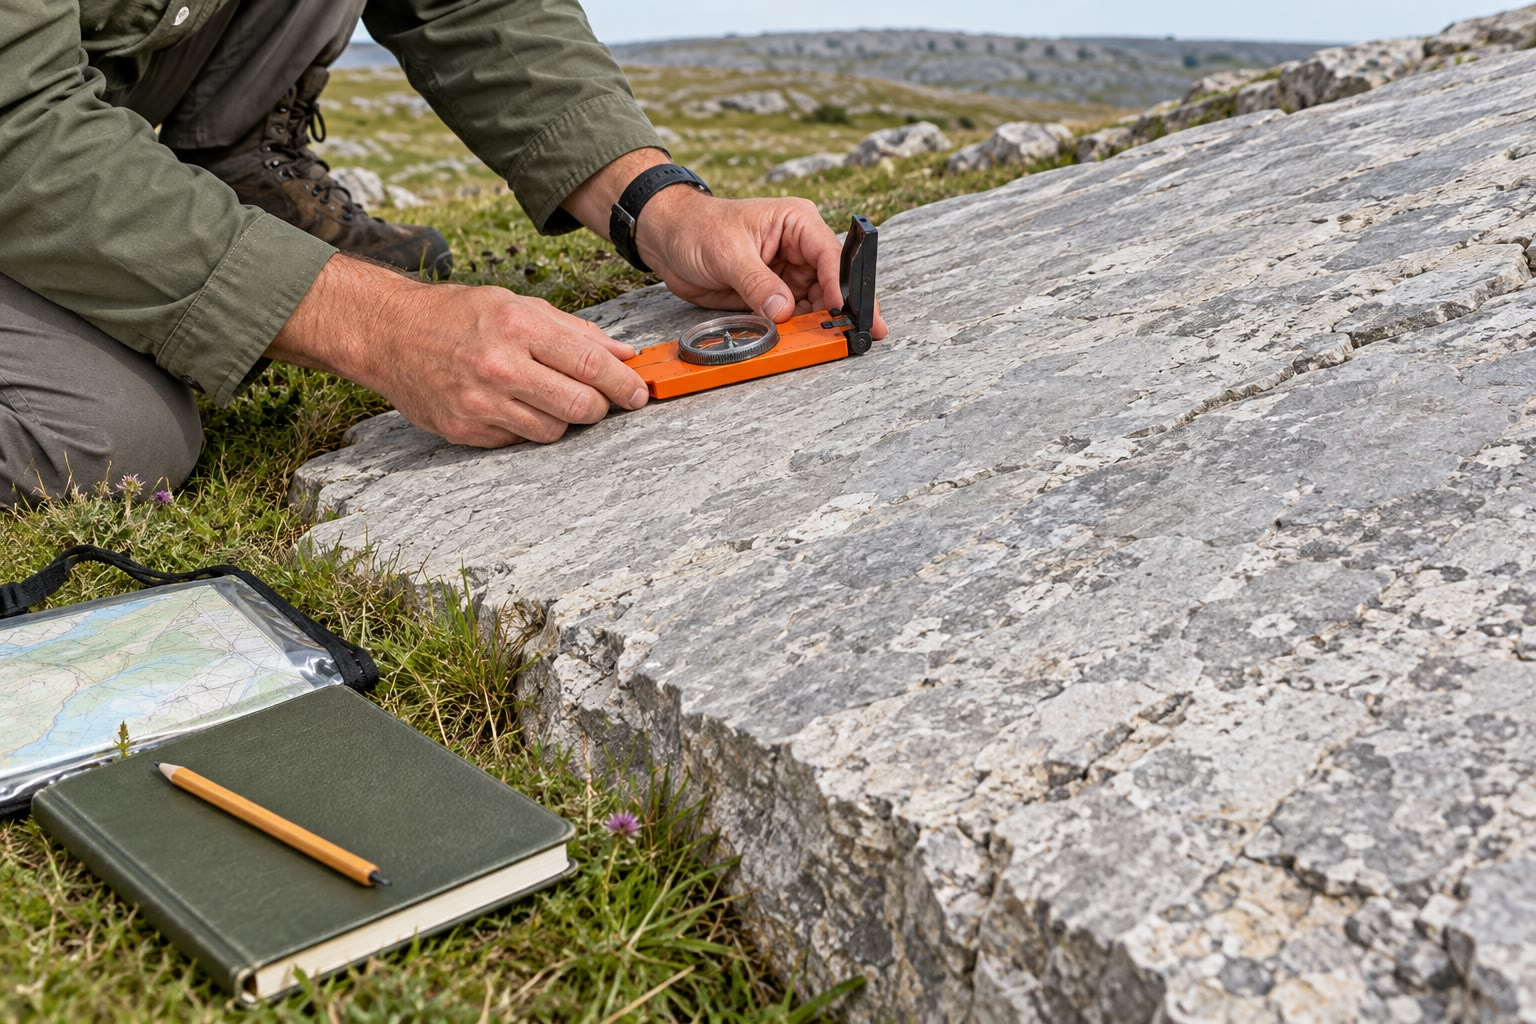
\includegraphics[width=0.6\linewidth]{images/book3/ai/b1-compass-clinometer.jpg}
\end{center}
\end{inthefield}

\begin{history}[El primer mapa geológico de un país]
% ledger: gsl:smith-1815, commons:smith-1815
El agrimensor William Smith, que excavó canales y drenó tierras en Inglaterra, observó que cada capa
de roca contenía sus propios fósiles, en un orden que era el mismo en todas partes. Usando los fósiles
para reconocer las capas, las siguió por el país durante más de quince años. Su mapa,
titulado \emph{A Delineation of the Strata of England and Wales, with part of
Scotland}, fechado el 1 de agosto de 1815, se considera el primer \omterm{def:b1:geological-maps:geological-map}{mapa geológico} de un país completo.
\begin{center}
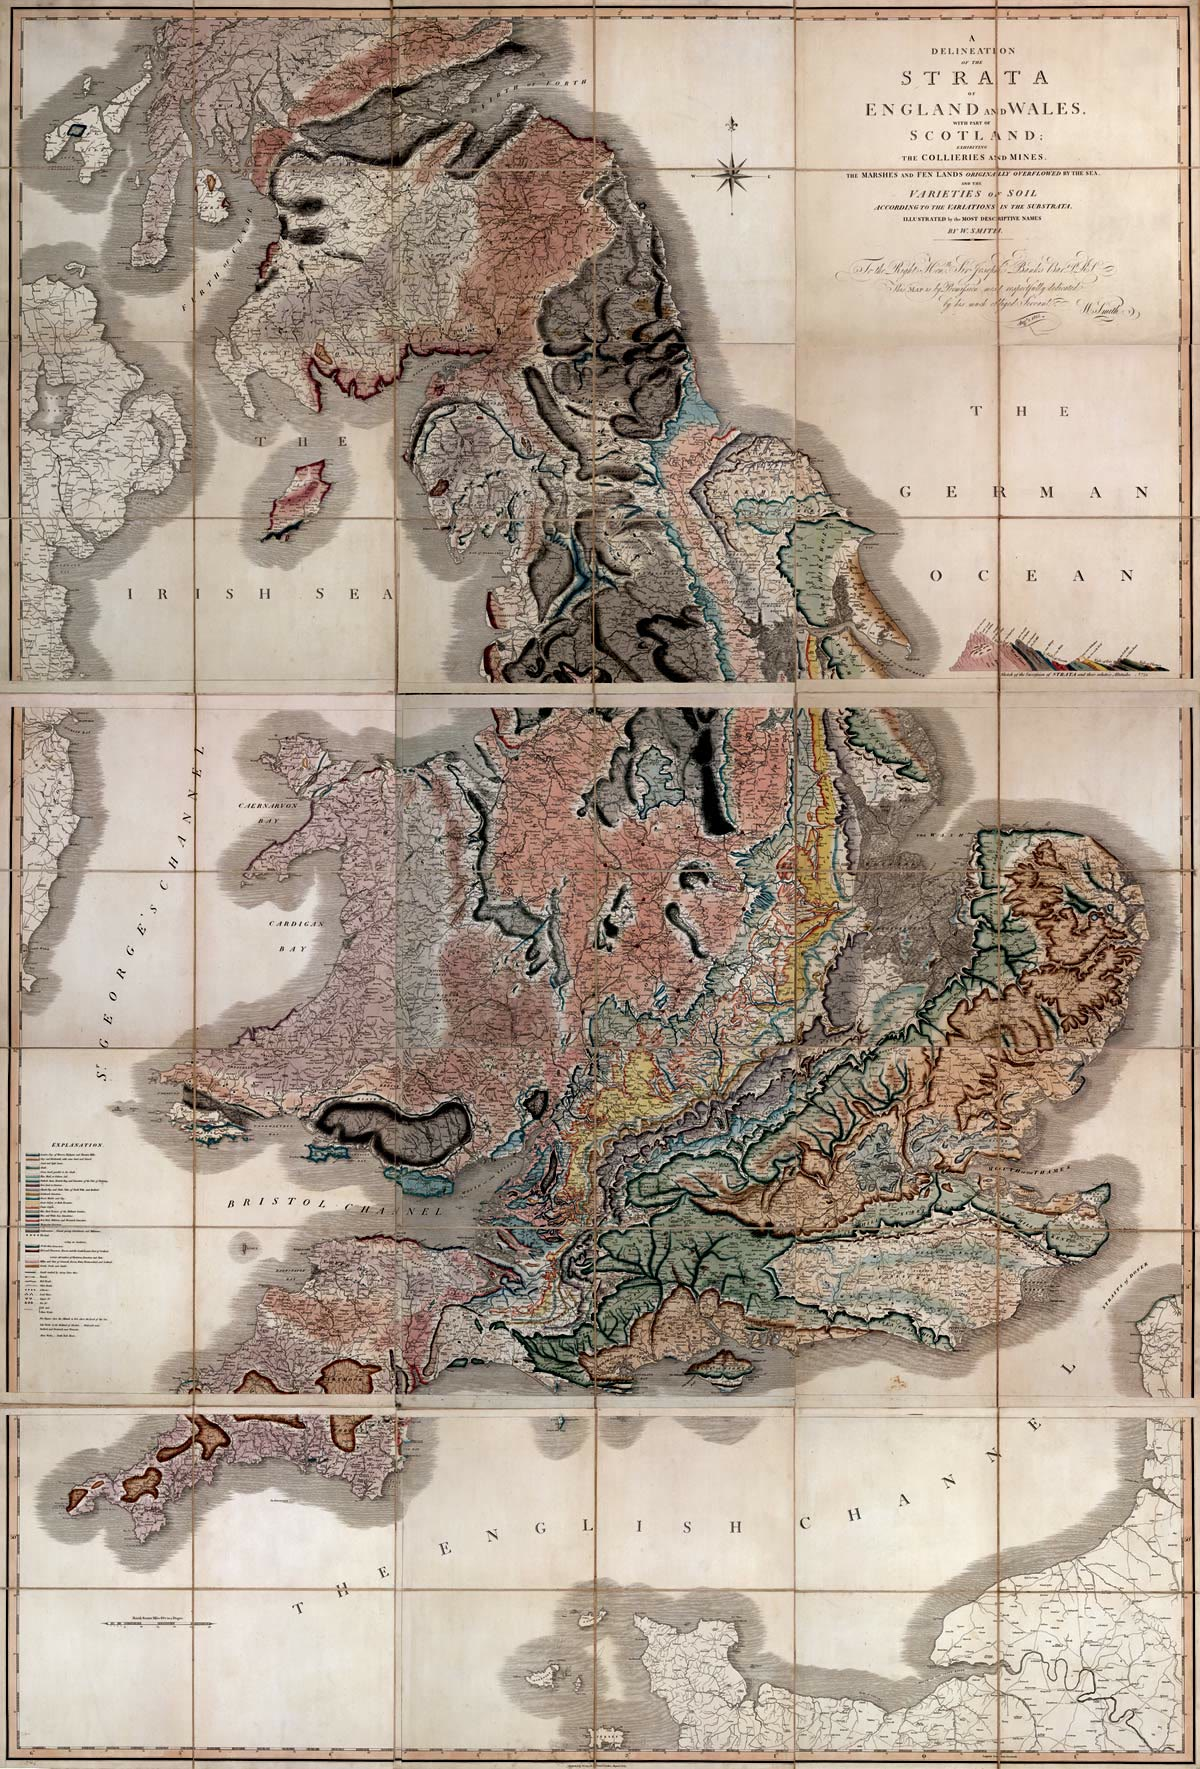
\includegraphics[width=0.36\linewidth]{images/book3/b1-smith-1815-map.jpg}

{\small Mapa de William Smith de 1815 (dominio público).}
\end{center}
\end{history}

\section{Ejercicios}

\begin{exercise}[$\star$]\label{exo:b1:geological-maps:1}
Defínanse el \omterm{def:b1:geological-maps:attitude}{rumbo}, el \omterm{def:b1:geological-maps:attitude}{buzamiento} y la \omterm{def:b1:geological-maps:attitude}{dirección de buzamiento} de un plano. Una capa tiene la
\omterm{def:b1:geological-maps:attitude}{actitud} $135/40$: calcúlese su \omterm{def:b1:geological-maps:attitude}{rumbo} según la regla de la mano derecha y dibújese su símbolo en el mapa.
\end{exercise}

\begin{exercise}[$\star$]\label{exo:b1:geological-maps:2}
Escríbase la ecuación del plano de \omterm{def:b1:geological-maps:attitude}{actitud} $090/30$ que pasa por el punto $(0, 0, 500)$, con
coordenadas en metros. ¿A qué altitud está en $(1000, 0)$ y en $(0, 1000)$?
\end{exercise}

\begin{exercise}[$\star$]\label{exo:b1:geological-maps:3}
En un mapa, la traza de un contacto sigue exactamente la curva de nivel de \qty{350}{m} a lo largo
de varios kilómetros de colinas y valles. ¿Qué puede decirse del contacto? ¿Y si su traza es una
recta que atraviesa colinas y valles?
\end{exercise}

\begin{exercise}[$\star$]\label{exo:b1:geological-maps:4}
En el mapa de las colinas de Varden, ¿qué unidad aflora en el núcleo del \omterm{def:b1:geological-maps:fold}{anticlinal} a lo largo del
río, y qué unidad ocupa el núcleo del \omterm{def:b1:geological-maps:fold}{sinclinal}? Explíquese por qué con el principio de superposición.
\end{exercise}

\begin{exercise}[$\star\star$]\label{exo:b1:geological-maps:5}
Un contacto se encuentra a las altitudes $\qty{300}{m}$ en $(0, 0)$, $\qty{300}{m}$ en $(1000, 0)$ y
$\qty{200}{m}$ en $(0, 500)$ (metros, $x$ hacia el este, $y$ hacia el norte). Calcúlense su \omterm{def:b1:geological-maps:attitude}{rumbo}, su
\omterm{def:b1:geological-maps:attitude}{dirección de buzamiento} y su \omterm{def:b1:geological-maps:attitude}{buzamiento}, primero razonando con las curvas de nivel de la estructura
y después con \cref{thm:b1:geological-maps:three-point}.
\end{exercise}

\begin{exercise}[$\star\star$]\label{exo:b1:geological-maps:6}
Un fondo de valle desciende hacia el norte a \qty{30}{m} por km. ¿Hacia qué lado apunta la V del
\omterm{def:b1:geological-maps:geological-map}{afloramiento} de un contacto si el contacto (a) es horizontal; (b) buza \ang{20} hacia el sur;
(c) buza \ang{1} hacia el norte; (d) buza \ang{20} hacia el norte? Justifíquese con
\cref{thm:b1:geological-maps:v-rule}.
\end{exercise}

\begin{exercise}[$\star\star$]\label{exo:b1:geological-maps:7}
En la situación de la regla de la V, un contacto buza aguas abajo con $a = 0.364$ (\ang{20}) y el
fondo del valle desciende con $s = 0.03$. Un punto del flanco del valle está \qty{80}{m} más alto
que el fondo. ¿A qué distancia aguas arriba del vértice está la traza en ese punto?
\end{exercise}

\begin{exercise}[$\star\star$]\label{exo:b1:geological-maps:8}
Los \omterm{def:b1:geological-maps:geological-map}{afloramientos} del \omterm{def:b1:geological-maps:fold}{anticlinal} de Varden se cierran alrededor del extremo norte de su núcleo.
¿En qué dirección se hunde el eje del \omterm{def:b1:geological-maps:fold}{pliegue}? ¿Se cierran los \omterm{def:b1:geological-maps:geological-map}{afloramientos} del \omterm{def:b1:geological-maps:fold}{sinclinal} al norte
o al sur?
\end{exercise}

\begin{exercise}[$\star\star$]\label{exo:b1:geological-maps:9}
En el \omterm{def:b1:geological-maps:geological-map}{mapa geológico}, a lo largo de la falla, ¿qué lado muestra en superficie unidades más jóvenes?
¿Qué bloque se hundió? Compruébese con el símbolo del mapa.
\end{exercise}

\begin{exercise}[$\star\star\star$]\label{exo:b1:geological-maps:10}
Demuéstrese que dos planos de \omterm{def:b1:geological-maps:attitude}{actitudes} $(\alpha_1, \delta_1)$ y $(\alpha_2, \delta_2)$ se cortan según
una recta paralela a $\vec n_1 \times \vec n_2$, donde $\vec n_i = (\tan\delta_i\sin\alpha_i,
\tan\delta_i\cos\alpha_i, 1)$. Aplíquese a los planos $090/30$ y $270/30$: ¿qué recta es, y qué tipo
de \omterm{def:b1:geological-maps:fold}{pliegue} forman los dos planos?
\end{exercise}

\begin{exercise}[$\star\star\star$]\label{exo:b1:geological-maps:11}
Un dique vertical tiene un \omterm{def:b1:geological-maps:attitude}{rumbo} de \ang{045} y aflora en el origen, sobre el fondo de un valle a la
altitud \qty{0}{m}. ¿Dónde puede estar su traza en una colina a \qty{300}{m}? Un segundo dique tiene
el mismo \omterm{def:b1:geological-maps:attitude}{rumbo}, buza \ang{60} hacia el sureste y también aflora en el origen. ¿A qué distancia del
origen, y en qué dirección, está su traza en un terreno a \qty{300}{m}, medida perpendicularmente al
\omterm{def:b1:geological-maps:attitude}{rumbo}?
\end{exercise}

\begin{exercise}[$\star\star\star$]\label{exo:b1:geological-maps:12}
En un \omterm{def:b1:geological-maps:dem}{modelo digital de elevaciones} con una malla de \qty{100}{m}, el terreno en $(x, y)$ y en
$(x + 100, y)$ está a 420 y \qty{405}{m}, y en $(x, y + 100)$ a \qty{412}{m}. Tratando el terreno de
esa celda como un plano, calcúlense su pendiente (en grados) y el \omterm{def:b1:spherical-astronomy:horizontal}{acimut} hacia el que mira
(dirección de la pendiente descendente).
\end{exercise}

\section{Problema: resolver las colinas de Varden}

\begin{problem}[{Problema de fin de semana --- de los sondeos y un mapa al eje del pliegue,
la falla y la historia de una región}]
\label{pb:b1:geological-maps:1}
% all data computed in figdata/bachelor-1/varden_maps.py from the region's
% model (figdata/shared/region.py); invented region: exercise data, no ledger
Una empresa que perfora pozos de agua en las colinas de Varden registra dónde sus sondeos
encuentran la base de la caliza; sus geólogos localizan también la falla donde cruza el terreno.
Las coordenadas están en metros al este y al norte de la esquina suroeste del mapa; las altitudes,
en metros sobre el nivel del mar. La parte I usa el \omterm{def:b1:geological-maps:geological-map}{mapa geológico} en color de
\cref{sec:b1:geological-maps:cut}.
\medskip
\noindent\textbf{Parte I --- Lectura del mapa.}
\begin{enumerate}
  \item Enumérense las unidades de la región de la más antigua a la más joven.
  \item ¿Qué unidades atraviesa el río, de oeste a este?
  \item ¿Qué unidad ocupa el núcleo del \omterm{def:b1:geological-maps:fold}{pliegue} cerca de $x = \qty{3.5}{km}$? ¿Qué tipo de \omterm{def:b1:geological-maps:fold}{pliegue} es?
  \item ¿Qué unidad ocupa el núcleo del \omterm{def:b1:geological-maps:fold}{pliegue} cerca de $x = \qty{7.5}{km}$? ¿Qué tipo de \omterm{def:b1:geological-maps:fold}{pliegue} es?
  \item ¿Por qué el esquisto y el granito solo son visibles cerca del río, en el núcleo del primer
        \omterm{def:b1:geological-maps:fold}{pliegue}?
  \item ¿Qué tipo de contacto separa la arenisca del granito? Justifíquese a partir del mapa.
\end{enumerate}

\medskip
\noindent Los sondeos (profundidad $d$ hasta la base de la caliza, altitud del terreno $z_g$) y los
tres puntos F1--F3 donde la falla cruza la parte superior del lecho rocoso (F2, en el valle, queda
bajo el aluvión delgado, que la falla no corta):

\begin{omfigure}
\begin{minipage}[c]{0.42\linewidth}
\centering\small
\begin{tabular}{lrrrr}
\hline
 & este & norte & $z_g$ & $d$ \\
\hline
E1 & 4000 & 6000 & 435 & 261 \\
E2 & 4600 & 7200 & 432 & 428 \\
E3 & 5100 & 6400 & 512 & 586 \\
W1 & 1500 & 6000 & 524 & 669 \\
W2 & 2200 & 7200 & 421 & 459 \\
W3 & 2600 & 5400 & 319 & 209 \\
\hline
 & este & norte & $z_g$ & \\
\hline
F1 & 4197 & 1000 & 405 & \\
F2 & 5824 & 3500 & 129 & \\
F3 & 7321 & 6500 & 482 & \\
\hline
\end{tabular}
\end{minipage}\hfill
\begin{minipage}[c]{0.56\linewidth}
\centering
\begin{tikzpicture}
\begin{axis}[axis equal image, xmin=0, xmax=10, ymin=0, ymax=8, width=\linewidth,
  tick label style={font=\scriptsize}, xlabel={este (km)}, ylabel={norte (km)},
  label style={font=\footnotesize}]
\addplot[fill=black!8, draw=black!50, line width=0.3pt, even odd rule] table {figdata/out/shared-region-unit-schist.dat};
\addplot[fill=black!8, draw=black!50, line width=0.3pt, even odd rule] table {figdata/out/shared-region-unit-granite.dat};
\addplot[fill=icsTriassic!20, draw=black!50, line width=0.3pt, even odd rule] table {figdata/out/shared-region-unit-sandstone.dat};
\addplot[fill=icsJurassic!25, draw=black!50, line width=0.3pt, even odd rule] table {figdata/out/shared-region-unit-limestone.dat};
\addplot[fill=icsJurassic!8, draw=black!50, line width=0.3pt, even odd rule] table {figdata/out/shared-region-unit-shale.dat};
\addplot[fill=icsCretaceous!20, draw=black!50, line width=0.3pt, even odd rule] table {figdata/out/shared-region-unit-chalk.dat};
\addplot[fault] table {figdata/out/shared-region-fault.dat};
\addplot[fill=omLithAlluv, draw=black!50, line width=0.3pt, even odd rule] table {figdata/out/shared-region-unit-alluvium.dat};
\addplot[river] table {figdata/out/shared-region-river.dat};
\addplot[only marks, mark=*, mark size=1.6pt] table[x=x_km, y=y_km] {figdata/out/bachelor-1-varden_maps-boreholes.dat};
\addplot[only marks, mark=square*, mark size=1.5pt, omThm] table[x=x_km, y=y_km] {figdata/out/bachelor-1-varden_maps-fault.dat};
\begin{scope}[every node/.style={font=\scriptsize\bfseries, inner sep=1.5pt, fill=white, fill opacity=0.8, text opacity=1}]
  \node[above right] at (axis cs:4,6) {E1};
  \node[above] at (axis cs:4.6,7.2) {E2};
  \node[right] at (axis cs:5.1,6.4) {E3};
  \node[above left] at (axis cs:1.5,6) {W1};
  \node[above] at (axis cs:2.2,7.2) {W2};
  \node[left] at (axis cs:2.6,5.4) {W3};
  \node[left, text=omThm] at (axis cs:4.197,1) {F1};
  \node[left, text=omThm] at (axis cs:5.824,3.5) {F2};
  \node[left, text=omThm] at (axis cs:7.321,6.5) {F3};
\end{scope}
\end{axis}
\end{tikzpicture}
\end{minipage}
\end{omfigure}

\medskip
\noindent\textbf{Parte II --- El flanco oriental.}
\begin{enumerate}[resume]
  \item Calcúlense las altitudes de la base de la caliza en E1, E2 y E3.
  \item Escríbanse los vectores $\overrightarrow{E_1E_2}$ y $\overrightarrow{E_1E_3}$.
  \item Calcúlese su producto vectorial y oriéntese hacia arriba.
  \item Dedúzcase el \omterm{def:b1:geological-maps:attitude}{buzamiento} de la base de la caliza en el flanco oriental.
  \item Dedúzcase su \omterm{def:b1:geological-maps:attitude}{dirección de buzamiento} y luego su \omterm{def:b1:geological-maps:attitude}{rumbo} según la regla de la mano derecha.
  \item ¿Es coherente el resultado con el símbolo de \omterm{def:b1:geological-maps:attitude}{rumbo} y \omterm{def:b1:geological-maps:attitude}{buzamiento} del flanco oriental en el mapa?
\end{enumerate}

\medskip
\noindent\textbf{Parte III --- El pliegue.}
\begin{enumerate}[resume]
  \item Calcúlense las altitudes de la base de la caliza en W1, W2 y W3.
  \item Calcúlese una normal hacia arriba $\vec n_W$ a la base de la caliza en el flanco occidental.
  \item Dedúzcase la \omterm{def:b1:geological-maps:attitude}{actitud} del flanco occidental.
  \item Calcúlese una dirección de la intersección de los dos flancos, el eje del \omterm{def:b1:geological-maps:fold}{pliegue}, como
        $\vec n_E \times \vec n_W$ (con $\vec n_E$ de la pregunta 9).
  \item Dése el \omterm{def:b1:geological-maps:attitude}{rumbo} (el \omterm{def:b1:spherical-astronomy:horizontal}{acimut} de la proyección horizontal del eje, tomado hacia abajo) y la
        inmersión (su ángulo bajo la horizontal) del eje del \omterm{def:b1:geological-maps:fold}{pliegue}.
  \item La base de la arenisca está sobre el eje a \qty{230}{m} donde el río lo cruza, cerca de
        $y = \qty{4}{km}$. ¿Cuánto más baja está sobre el eje \qty{8}{km} más al norte? ¿Es coherente
        esto con la pregunta 3 de la parte I y con el cierre de los \omterm{def:b1:geological-maps:geological-map}{afloramientos}?
\end{enumerate}

\medskip
\noindent\textbf{Parte IV --- La falla y la historia.}
\begin{enumerate}[resume]
  \item A partir de F1, F2 y F3, calcúlese la \omterm{def:b1:geological-maps:attitude}{actitud} de la falla.
  \item A lo largo de la falla, las unidades en superficie del lado este-sureste son más jóvenes que
        las que tienen enfrente. ¿Qué bloque se hundió? ¿Es la falla normal o inversa?
  \item La recta de F1 a F3 pasa unos \qty{200}{m} al oeste de F2. ¿Por qué la traza de la falla se
        curva hacia el este-sureste al cruzar el valle del río, en F2?
  \item Póngase en orden: plegamiento; sedimentación de la creta; fallamiento; intrusión del granito;
        erosión antes de la arenisca; sedimentación del aluvión.
  \item La creta tiene 90 millones de años y está plegada; el aluvión se depositó en los últimos
        2.58 millones de años y no está fallado. ¿Entre qué edades tuvieron lugar el plegamiento y el
        fallamiento?
  \item Para alcanzar la falla a \qty{1000}{m} bajo el nivel del mar bajo F1, ¿a qué distancia de F1 y
        en qué dirección debe perforarse un pozo vertical?
\end{enumerate}
\end{problem}
